\documentclass[a4paper, 11pt]{article}
\usepackage{amsmath}
\usepackage{graphicx}
\usepackage{geometry}
\usepackage{color}
\usepackage{listings}
\definecolor{dkgreen}{rgb}{0,0.6,0}
\definecolor{gray}{rgb}{0.5,0.5,0.5}
\definecolor{mauve}{rgb}{0.58,0,0.82}
\lstset{frame=shadowbox,
    language=Python,
    aboveskip=3mm,
    belowskip=3mm,
    showstringspaces=false,
    columns=flexible,
    basicstyle={\small\ttfamily},
    numbers=left,
    numberstyle=\tiny\color{gray},
    keywordstyle=\color{blue},
    commentstyle=\color{dkgreen},
    stringstyle=\color{mauve},
    breaklines=true,
    breakatwhitespace=true,
    tabsize=3
}
\usepackage[colorlinks,linkcolor=red]{hyperref}
\geometry{scale=0.8}
\linespread{1.5}
\usepackage{hyperref}

\title{	
\normalfont \normalsize
\textsc{School of Data and Computer Science, Sun Yat-sen University} \\ [25pt] %textsc small capital letters
\rule{\textwidth}{0.5pt} \\[0.4cm] % Thin top horizontal rule
\huge  E04 Futoshiki Puzzle ( Forward Checking)\\ % The assignment title
\rule{\textwidth}{2pt} \\[0.5cm] % Thick bottom horizontal rule
\author{17341203 Yixin Zhang}
\date{\normalsize\today}
}

\begin{document}
\maketitle
\tableofcontents
\newpage

\section{Futoshiki}
Futoshiki is a board-based puzzle game, also known under the name Unequal. It is playable on a square board having a given fixed size ($4\times4$ for example).

The purpose of the game is to discover the digits hidden inside the board's cells; each cell is filled with a digit between 1 and the board's size. On each row and column each digit appears exactly once; therefore, when revealed, the digits of the board form a so-called Latin square.

At the beginning of the game some digits might be revealed. The board might also contain some inequalities between the board cells; these inequalities must be respected and can be used as clues in order to discover the remaining hidden digits.

Each puzzle is guaranteed to have a solution and only one.

You can play this game online: \url{http://www.futoshiki.org/}.
\begin{figure}[h]
  \centering
  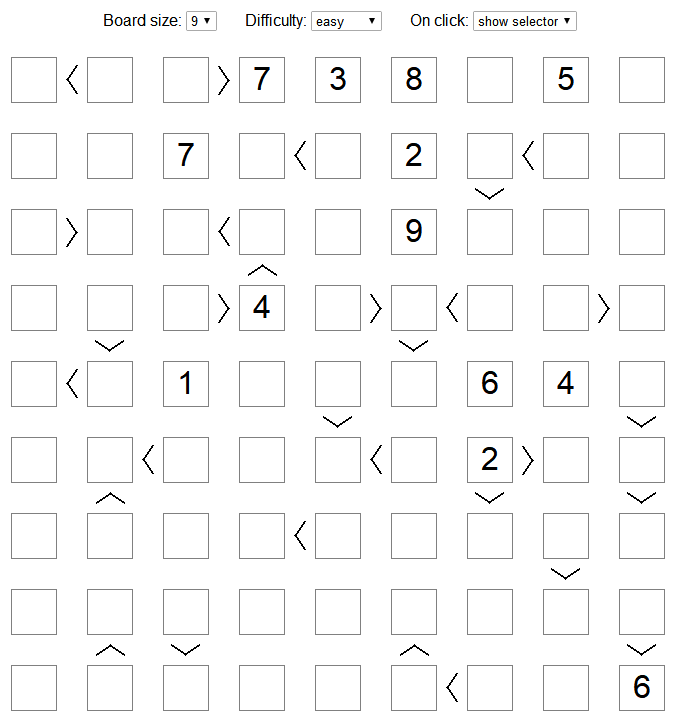
\includegraphics[width=7.5cm]{Pic/futoshiki1}
  \qquad
  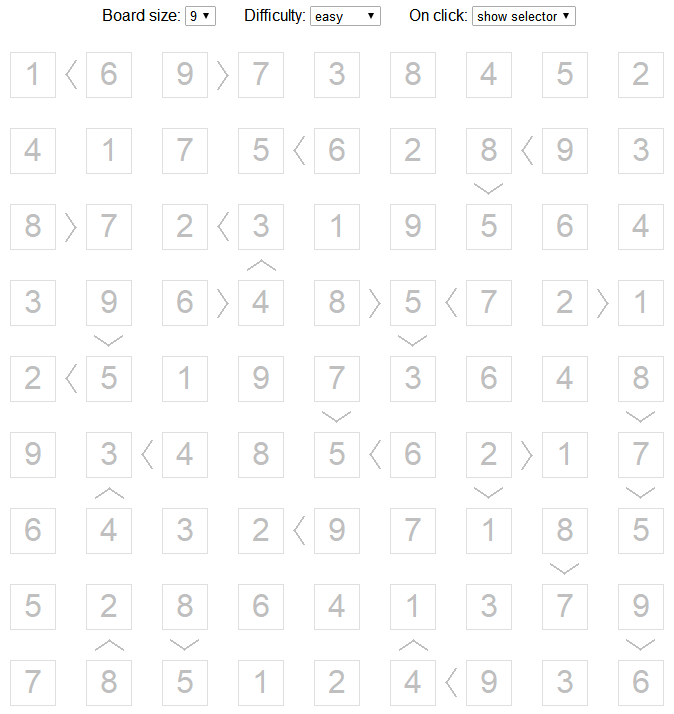
\includegraphics[width=7.5cm]{Pic/futoshiki2}
  \label{fig:puzzle}
  \caption{An Futoshiki Puzzle}
\end{figure}

\section{Tasks}


\begin{enumerate}
\item Please solve the above Futoshiki puzzle ( Figure \ref{fig:puzzle} ) with forward checking algorithm.
\item Write the related codes and take a screenshot of the running results in the file named \textsf{E04\_YourNumber.pdf}, and send it to \textsf{ai\_201901@foxmail.com}.

\end{enumerate}
\section{Basic Backtrack}
\subsection{Overview}
Here I've tried to use basic backtrack algorithm to solve this problem. No optimization is made. I wrote this code because I want to make a comparison with forward checking algorithm.

\subsection{Python Code}

\begin{lstlisting}[title=basic_backtrack.py]
# @Author: Jed Zhang
# @Date: 2019-09-19 16:33:50
# @Last Modified by:   Jed Zhang
# @Last Modified time: 2019-09-19 16:33:50

import numpy as np
import copy

SIZE = -1


def isSolved(puzzle):
    """
    Check whether all cells in the puzzle is filled.
    """
    return puzzle.all()  # test if all values are non-zero


def isValid(puzzle, constraints):
    """
    Check whether all constraints are satisfied.
    """
    s = set()

    # rows
    for i in range(SIZE):
        for j in range(SIZE):
            if puzzle[i, j] != 0 and puzzle[i, j] in s:
                return False  # duplicated in row
            else:
                s.add(puzzle[i, j])
        s.clear()

    # columns
    for j in range(SIZE):
        for i in range(SIZE):
            if puzzle[i, j] != 0 and puzzle[i, j] in s:
                return False  # duplicated in row
            else:
                s.add(puzzle[i, j])
        s.clear()

    # constraints
    for constraint in constraints:
        large = puzzle[constraint[0], constraint[1]]
        small = puzzle[constraint[2], constraint[3]]
        if large != 0 and small != 0 and not large > small:
            return False

    # pass all tests, so it is valid
    return True


def basicBacktrack(puzzle_origin, constraints):
    """
    Basic backtrack (without forward checking).
    If a solution is found, return it; else return None.
    """
    puzzle = puzzle_origin.copy()  # the origin puzzle is not modified

    if isSolved(puzzle):
        return puzzle

    pos = np.where(puzzle == 0)
    pos = pos[0][0], pos[1][0]  # position of the first empty cell

    for i in range(1, SIZE + 1):
        puzzle[pos] = i
        if isValid(puzzle, constraints):
            ret = basicBacktrack(puzzle, constraints)
            if ret is not None:
                return ret

    puzzle[pos] = 0  # restore the assignment
    return None


def loadFutoshiki(puz_filename, con_filename):
    """
    Read the puzzle and constraints from files to numpy matrices,
    and convert the coordinates into 0-indexed (coordinates in the
    file are 1-indexed).
    """
    global SIZE
    puzzle = np.loadtxt(puz_filename, dtype=np.uint8)
    constraints = np.loadtxt(con_filename, dtype=np.uint8) - 1  # index start at 0 instead of 1
    SIZE = len(puzzle)  # the side length of the puzzle
    return puzzle, constraints


if __name__ == '__main__':
    # basic backtrack runs slowly, so we use a small puzzle (5x5) to test it
    puzzle, constraints = loadFutoshiki('smallpuzzle.txt', 'smallconstraints.txt')
    result = basicBacktrack(puzzle, constraints)

    if result is not None:
        print('Solution found:')
        print(result)
    else:
        print('[-] No solution!')
\end{lstlisting}

\subsection{Result}
The code is able to output the correct solution on small puzzles. However, it takes forever to solve the problem at a bigger size, such as a 9*9 puzzle.

\section{Forward Checking}
\subsection{Overview}
Based on basic backtrack code above, I added forward checking and MRV into it. Every time a new variable is assigned, all values that violate the constraints will be removed from their domains.


Using the same idea, I implement the algorithm in both Python and C++. My purpose is still to compare.

Since this report is the second one (I have submitted one several hours ago), I would like to talk about the optimization that I've made in this newer version. I wrote a new function `domainCount()', which counts the total number of values available in each variable's domain. While initializing the domains, I use a do-while loop to update domains several times, until the return value of `domainCount()' cannot decrease anymore. With this procedure, the state space can be minimized before doing forward checking. According to the results, this optimization can make the calculation many times faster.

\subsection{Python Code}

\begin{lstlisting}[title=python/forward\_checking.py]
# @Author: Jed Zhang
# @Date: 2019-09-19 16:33:50
# @Last Modified by:   Jed Zhang
# @Last Modified time: 2019-09-19 16:33:50

import numpy as np
import copy
from pprint import pprint

SIZE = -1


def isSolved(puzzle):
    """
    Check whether all cells in the puzzle is filled.
    """
    return puzzle.all()  # test if all values are non-zero


def makeDomains(puzzle, constraints):
    """
    Make a dict as the initial domains of all variables. This function
    should be called only once at the beginning of the program.
    """

    def domainCount(domains):
        """
        Count the total number of values available in the puzzle.
        """
        count = 0
        for domain in domains.values():
            count += len(domain)
        return count

    # initialize
    domains = {}
    for i in range(SIZE):
        for j in range(SIZE):
            if puzzle[i, j] != 0:
                domains[i, j] = {puzzle[i, j]}
            else:
                domains[i, j] = set(range(1, SIZE + 1))

    # remove values that have conflict on rows or columns
    for i in range(SIZE):
        for j in range(SIZE):
            if puzzle[i, j] != 0:
                for i2 in range(SIZE):
                    if i2 != i and puzzle[i, j] in domains[i2, j]:
                        domains[i2, j].remove(puzzle[i, j])
                        if len(domains[i2, j]) == 0:
                            return None  # DWO
                for j2 in range(SIZE):
                    if j2 != j and puzzle[i, j] in domains[i, j2]:
                        domains[i, j2].remove(puzzle[i, j])
                        if len(domains[i, j2]) == 0:
                            return None  # DWO

    # remove values that have conflict with constraints
    old_domain_count = 0
    while True:
        # repeat until total count of all domains cannot decrease anymore
        # I think this procedure can reduce the state space, thus speed up the search
        for constraint in constraints:
            large_pos = (constraint[0], constraint[1])
            small_pos = (constraint[2], constraint[3])
            if puzzle[large_pos] != 0:  # large_pos has been assigned
                for i in range(puzzle[large_pos], SIZE + 1):
                    if i in domains[small_pos]:
                        domains[small_pos].remove(i)
                        if len(domains[small_pos]) == 0:
                            return None  # DWO
            else:  # large_pos has not been assigned
                minimum = min(domains[small_pos])
                if minimum in domains[large_pos]:
                    domains[large_pos].remove(minimum)


            if puzzle[small_pos] != 0:  # small_pos has been assigned
                for i in range(1, puzzle[small_pos] + 1):
                    if i in domains[large_pos]:
                        domains[large_pos].remove(i)
                        if len(domains[large_pos]) == 0:
                            return None  # DWO
            else:  # small_pos has not been assigned
                maximum = max(domains[large_pos])
                if maximum in domains[small_pos]:
                    domains[small_pos].remove(maximum)

        # repeat ends
        new_domain_count = domainCount(domains)
        if new_domain_count == old_domain_count:
            break
        else:
            old_domain_count = new_domain_count


    return domains


def updateDomains(puzzle, constraints, domains_origin, pos):
    """
    In each iteration, we have chosen a pos using MRV, and assign a
    value in its domain to it. After that, we have to update some
    variables' domains by removing some values which has conflict with
    the assignment.
    """
    domains = copy.deepcopy(domains_origin)  # deep copy

    # check the same column
    for i in range(SIZE):
        if i == pos[0]:
            continue
        if puzzle[i, pos[1]] == puzzle[pos]:
            return None
        if puzzle[pos] in domains[i, pos[1]]:
            domains[i, pos[1]].remove(puzzle[pos])
            if len(domains[i, pos[1]]) == 0:
                return None  # DWO

    # check the same row
    for j in range(SIZE):
        if j == pos[1]:
            continue
        if puzzle[pos[0], j] == puzzle[pos]:
            return None
        if puzzle[pos] in domains[pos[0], j]:
            domains[pos[0], j].remove(puzzle[pos])
            if len(domains[pos[0], j]) == 0:
                return None  # DWO

    # check the constraints
    for constraint in constraints:
        large_pos = (constraint[0], constraint[1])
        small_pos = (constraint[2], constraint[3])
        if pos == large_pos:
            for k in range(puzzle[pos], SIZE + 1):
                if k in domains[small_pos]:
                    domains[small_pos].remove(k)
                    if len(domains[small_pos]) == 0:
                        return None  # DWO
        elif pos == small_pos:
            for k in range(1, puzzle[pos] + 1):
                if k in domains[large_pos]:
                    domains[large_pos].remove(k)
                    if len(domains[large_pos]) == 0:
                        return None  # DWO
    return domains


def mrv(puzzle, domains):
    """
    Find the variable with minimum remaining values (MRV),
    and return its position.
    """
    min_val = SIZE * SIZE  # max size of domain
    min_pos = (-1, -1)
    for i in range(SIZE):
        for j in range(SIZE):
            if puzzle[i, j] == 0 and len(domains[i, j]) < min_val:
                min_val = len(domains[i, j])
                min_pos = (i, j)
    return min_pos


def forwardChecking(puzzle_origin, constraints, domains_origin):
    """
    Use forward checking algorithm to solve the CSP problem.
    """
    puzzle = puzzle_origin.copy()
    domains = domains_origin.copy()

    if isSolved(puzzle):
        return puzzle

    pos = mrv(puzzle, domains)  # find a unassigned variable using MRV

    for d in domains[pos]:
        puzzle[pos] = d
        temp_domains = updateDomains(puzzle, constraints, domains, pos)
        if temp_domains is not None:  # not DWO
            ret = forwardChecking(puzzle, constraints, temp_domains)
            if ret is not None:
                return ret

    puzzle[pos] = 0  # restore the assignment
    return None


def loadFutoshiki(puz_filename, con_filename):
    """
    Read the puzzle and constraints from files to numpy matrices,
    and convert the coordinates into 0-indexed (coordinates in the
    file are 1-indexed).
    """
    global SIZE
    puzzle = np.loadtxt(puz_filename, dtype=np.uint8)
    constraints = np.loadtxt(con_filename, dtype=np.uint8) - 1  # index start at 0 instead of 1
    SIZE = len(puzzle)  # the side length of the puzzle
    return puzzle, constraints


if __name__ == '__main__':
    puzzle, constraints = loadFutoshiki('../puzzle.txt', '../constraints.txt')
    domains = makeDomains(puzzle, constraints)
    result = forwardChecking(puzzle, constraints, domains)

    if result is not None:
        print('Solution found:')
        print(result)
    else:
        print('[-] No solution!')
\end{lstlisting}


\subsection{C++ Code}
\begin{lstlisting}[title=cpp/forward_checking.cpp]
#include <fstream>
#include <iostream>
#include <map>
#include <set>
#include <string>
#include <vector>
using namespace std;

class Futoshiki {
public:
    int size;
    int con_num;
    vector<vector<int>> puzzle;
    vector<pair<pair<int, int>, pair<int, int>>> constraints;

    Futoshiki(const char* puz_filename, const char* con_filename, int size, int con_num);                 // read puzzle and constraints from file
    bool isSolved();                                                                                      // check whether the puzzle is solved
    vector<vector<set<int>>> makeDomains();                                                               // initialize the domains of each variable
    vector<vector<set<int>>> updateDomains(vector<vector<set<int>>> domains, const pair<int, int>& pos);  // update each domain after assigning a variable
    pair<int, int> mrv(const vector<vector<set<int>>>& domains);                                          // choose a unassigned variable with minimum remaining values
    vector<vector<int>> forwardChecking(const vector<vector<set<int>>>& domains);                         // try to solve the CSP

private:
    // count the total number of values available in the puzzle
    int domainCount(const vector<vector<set<int>>>& domains) {
        int count = 0;
        for(int i = 0; i < size; i++) {
            for(int j = 0; j < size; j++) {
                count += domains[i][j].size();
            }
        }
        return count;
    }
};

/*
    Read the puzzle and constraints from files to numpy matrices,
    and convert the coordinates into 0-indexed (coordinates in the
    file are 1-indexed).
*/
Futoshiki::Futoshiki(const char* puz_filename, const char* con_filename, int size, int con_num)
    : size(size), con_num(con_num), puzzle(size, vector<int>(size, 0)) {
    ifstream puz_file(puz_filename), con_file(con_filename);
    for (int i = 0; i < size; i++) {
        for (int j = 0; j < size; j++) {
            puz_file >> puzzle[i][j];
        }
    }

    for (int i = 0; i < con_num; i++) {
        int x1, y1, x2, y2;
        con_file >> x1 >> y1 >> x2 >> y2;
        constraints.push_back(make_pair(make_pair(x1 - 1, y1 - 1), make_pair(x2 - 1, y2 - 1)));
    }
    puz_file.close();
    con_file.close();
}

/* Check whether all cells in the puzzle is filled. */
bool Futoshiki::isSolved() {
    for (int i = 0; i < puzzle.size(); i++) {
        for (int j = 0; j < puzzle[0].size(); j++) {
            if (puzzle[i][j] == 0) {
                return false;
            }
        }
    }
    return true;
}

vector<vector<set<int>>> Futoshiki::makeDomains() {
    // initialize
    vector<vector<set<int>>> domains(size, vector<set<int>>(size, set<int>()));
    for (int i = 0; i < size; i++) {
        for (int j = 0; j < size; j++) {
            if (puzzle[i][j] == 0) {
                for (int k = 0; k < size; k++) {
                    domains[i][j].insert(k + 1);
                }
            } else {
                domains[i][j].insert(puzzle[i][j]);
            }
        }
    }

    // remove values that have conflict on rows or columns
    for (int i = 0; i < size; i++) {
        for (int j = 0; j < size; j++) {
            if (puzzle[i][j] != 0) {
                for (int i2 = 0; i2 < size; i2++) {
                    if (i2 != i) {
                        domains[i2][j].erase(puzzle[i][j]);
                    }
                }
                for (int j2 = 0; j2 < size; j2++) {
                    if (j2 != j) {
                        domains[i][j2].erase(puzzle[i][j]);
                    }
                }
            }
        }
    }

    // remove values that have conflict with constraints
    int old_domain_count = 0, new_domain_count;
    // repeat until total count of all domains cannot decrease anymore
    do {
        for (int i = 0; i < con_num; i++) {
            pair<int, int> large_pos = constraints[i].first;
            pair<int, int> small_pos = constraints[i].second;
            if (puzzle[large_pos.first][large_pos.second] != 0) {  // large_pos has been assigned
                for (int k = puzzle[large_pos.first][large_pos.second]; k <= size; k++) {
                    domains[small_pos.first][small_pos.second].erase(k);
                }
            }
            else {  // large_pos has not been assigned
                int minimum = *domains[small_pos.first][small_pos.second].begin();
                domains[large_pos.first][large_pos.second].erase(minimum);
            }
            if (puzzle[small_pos.first][small_pos.second] != 0) {
                for (int k = 1; k <= puzzle[small_pos.first][small_pos.second]; k++) {
                    domains[large_pos.first][large_pos.second].erase(k);
                }
            }
            else {
                int minimum = *domains[large_pos.first][large_pos.second].rbegin();
                domains[small_pos.first][small_pos.second].erase(minimum);
            }
        }
        new_domain_count = domainCount(domains);
    } while(old_domain_count == new_domain_count);

    return domains;
}

/*
    In each iteration, we have chosen a pos using MRV, and assign a
    value in its domain to it. After that, we have to update some
    variables` domains by removing some values which has conflict with
    the assignment.
*/
vector<vector<set<int>>> Futoshiki::updateDomains(vector<vector<set<int>>> domains, const pair<int, int>& pos) {
    // check the same column
    for (int i = 0; i < size; i++) {
        if (i == pos.first)
            continue;
        else if (puzzle[i][pos.second] == puzzle[pos.first][pos.second]) {
            return vector<vector<set<int>>>();  // DWO
        } else {
            domains[i][pos.second].erase(puzzle[pos.first][pos.second]);
            if (domains[i][pos.second].size() == 0) {
                return vector<vector<set<int>>>();  // DWO
            }
        }
    }

    // check the same row
    for (int j = 0; j < size; j++) {
        if (j == pos.second)
            continue;
        else if (puzzle[pos.first][j] == puzzle[pos.first][pos.second]) {
            return vector<vector<set<int>>>();  // DWO
        } else {
            domains[pos.first][j].erase(puzzle[pos.first][pos.second]);
            if (domains[pos.first][j].size() == 0) {
                return vector<vector<set<int>>>();  // DWO
            }
        }
    }

    // check the constraints
    for (int i = 0; i < con_num; i++) {
        pair<int, int> large_pos = constraints[i].first;
        pair<int, int> small_pos = constraints[i].second;
        if (pos == large_pos) {
            for (int k = puzzle[pos.first][pos.second]; k <= size; k++) {
                domains[small_pos.first][small_pos.second].erase(k);
                if (puzzle[small_pos.first][small_pos.second] == 0 && domains[small_pos.first][small_pos.second].size() == 0) {
                    return vector<vector<set<int>>>();  // DWO
                }
            }
        } else if (pos == small_pos) {
            for (int k = 1; k <= puzzle[pos.first][pos.second]; k++) {
                domains[large_pos.first][large_pos.second].erase(k);
                if (puzzle[large_pos.first][large_pos.second] == 0 && domains[large_pos.first][large_pos.second].size() == 0) {
                    return vector<vector<set<int>>>();  // DWO
                }
            }
        }
    }
    return domains;
}

/*
    Find the variable with minimum remaining values (MRV),
    and return its position.
*/
pair<int, int> Futoshiki::mrv(const vector<vector<set<int>>>& domains) {
    int min_val = size * size;  // max size of domain
    pair<int, int> min_pos = make_pair(-1, -1);
    for (int i = 0; i < size; i++) {
        for (int j = 0; j < size; j++) {
            if (puzzle[i][j] == 0 && domains[i][j].size() < min_val) {
                min_val = domains[i][j].size();
                min_pos = make_pair(i, j);
            }
        }
    }
    return min_pos;
}

/* Use forward checking algorithm to solve the CSP problem. */
vector<vector<int>> Futoshiki::forwardChecking(const vector<vector<set<int>>>& domains) {
    if (isSolved()) {
        return puzzle;
    }

    pair<int, int> pos = mrv(domains);

    for (auto pd = domains[pos.first][pos.second].begin(); pd != domains[pos.first][pos.second].end(); pd++) {
        puzzle[pos.first][pos.second] = *pd;
        auto temp_domains = updateDomains(domains, pos);
        if (temp_domains.size() != 0) {  // not DWO
            vector<vector<int>> ret = forwardChecking(temp_domains);
            if (ret.size() != 0) return ret;
        }
    }

    puzzle[pos.first][pos.second] = 0;  // restore the assignment
    return vector<vector<int>>();
}

int main() {
    Futoshiki game("../puzzle.txt", "../constraints.txt", 9, 30);
    auto domains = game.makeDomains();
    vector<vector<int>> result = game.forwardChecking(domains);
    if (result.size() != 0) {
        cout << "Solution found:" << endl;
        for (int i = 0; i < game.size; i++) {
            for (int j = 0; j < game.size; j++) {
                cout << result[i][j] << " ";
            }
            cout << endl;
        }
    } else {
        cout << "[-] No solution!" << endl;
    }
    return 0;
}
\end{lstlisting}
\subsection{Result}
Both Python implementation and C++ implementation can produce correct result, but C++ is much faster than Python. The Python code takes about 25 seconds to solve a 9*9 puzzle, while the C++ code takes only 1 seconds.

\begin{figure}[ht]
\centering
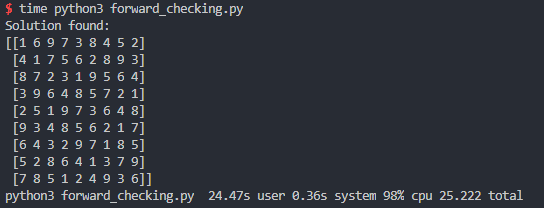
\includegraphics[scale=0.9]{pyresult.png}
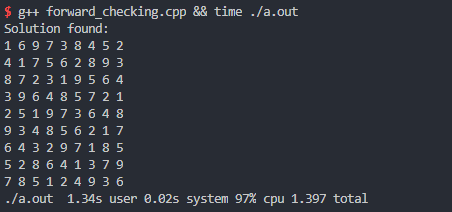
\includegraphics[scale=0.9]{cppresult.png}
\end{figure}

\section{Discussion}
After four experiments, I can clearly feel the difference in speed between Python and C++. Writing Python code is definitely a pleasure, but it is really slow. C++ is faster, but you need to pay more attention while writing code, especially when using STL.

The optimazation that I have made in this second version is really effective. It makes the algorithm about 50 times faster. Actually, the searching procedure has not been optimized. It is the initial state space that has been minimized.

%\clearpage
%\bibliography{E:/Papers/LiuLab}
%\bibliographystyle{apalike}
\end{document} 
%%% Local Variables:
%%% mode: latex
%%% TeX-master: t
%%% End:
